% 2001 年全国新课程卷理科第 20 题甲：正四棱锥坐标图
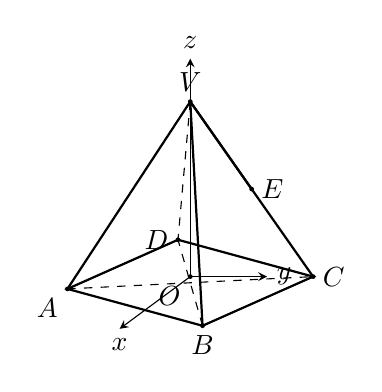
\begin{tikzpicture}[>=stealth, scale=0.78]
  \coordinate (A) at (-2.0,-0.4);
  \coordinate (B) at (0.2,-1.0);
  \coordinate (C) at (2.0,-0.2);
  \coordinate (D) at (-0.2,0.4);
  \coordinate (O) at (0, -0.2);
  \coordinate (V) at (0,2.65);
  \coordinate (E) at (1.0,1.225);

  \draw[thick] (A)--(B)--(C)--(D)--cycle;
  \draw[dashed] (A)--(C) (B)--(D);
  \draw[thick] (V)--(A) (V)--(B) (V)--(C);
  \draw[dashed] (V)--(D);
  \draw[thick] (V)--(E);
  \fill (A) circle (1.1pt) node[below left] {$A$};
  \fill (B) circle (1.1pt) node[below] {$B$};
  \fill (C) circle (1.1pt) node[right] {$C$};
  \fill (D) circle (1.1pt) node[left] {$D$};
  \fill (O) circle (1.1pt) node[below left] {$O$};
  \fill (V) circle (1.1pt) node[above] {$V$};
  \fill (E) circle (1.1pt) node[right] {$E$};
  \draw[->] (O)--(-1.15,-1.05) node[below] {$x$};
  \draw[->] (O)--(1.25,-0.2) node[right] {$y$};
  \draw[->] (O)--(0,3.35) node[above] {$z$};
\end{tikzpicture}
